% Figure snippets for sex-specific-resilience manuscript.

% Figure: Experimental schema
\begin{figure}[htbp]
\centering
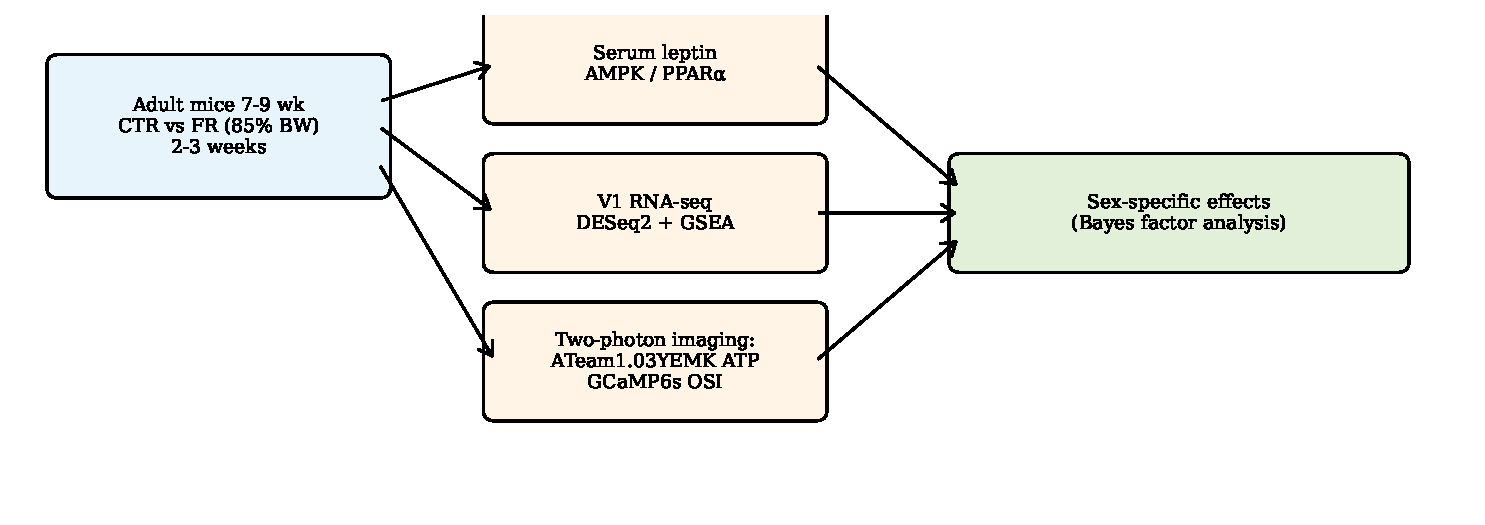
\includegraphics[width=0.9\textwidth]{figures/fig_schema_experiment.pdf}
\caption{Experimental pipeline. Adult male and female mice (7--9 weeks) were either fed ad libitum (CTR) or food-restricted (FR) to 85\% of free-feeding bodyweight for 2--3 weeks. V1 tissue was analysed for serum leptin, AMPK Thr172 phosphorylation, PPAR$\alpha$ DNA binding, and bulk RNA sequencing (DESeq2 and GSEA). In parallel, two-photon FRET imaging of ATeam1.03YEMK reported cortical ATP usage and GCaMP6s imaging reported orientation selectivity of V1 layer 2/3 neurons. Sex-specific effects were assessed with two-way ANOVA and Bayes factor analysis.}
\label{fig:schema}
\end{figure}

% Figure 1: Weight, leptin, AMPK, PPARalpha
\begin{figure}[htbp]
\centering
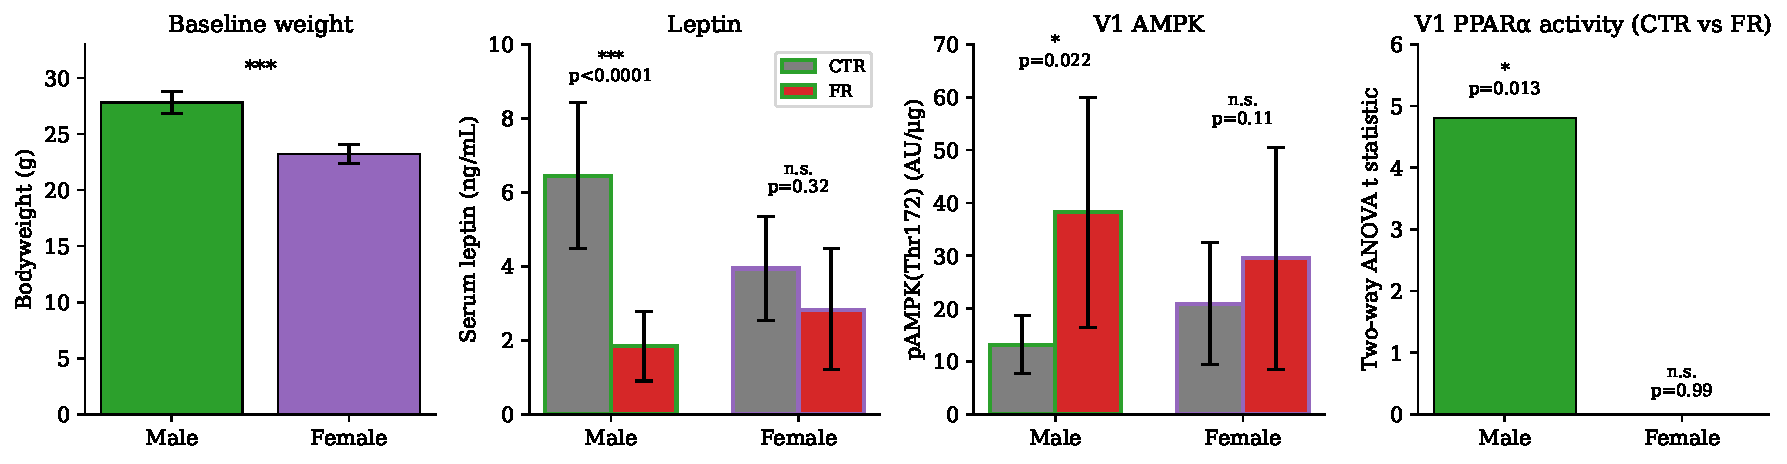
\includegraphics[width=\textwidth]{figures/fig1_weight_leptin_ampk.pdf}
\caption{Sex-specific impact of food restriction on body composition and V1 energy-regulating pathways. Baseline bodyweight differed by sex (males 27.82~g [95\% CI 26.84--28.79] vs females 23.21~g [22.35--24.07]; $t=7.58$, $df=66$, $p<0.001$). Serum leptin dropped from 6.45~ng/mL [4.47--8.43] to 1.84~ng/mL [0.90--2.79] in males ($t=4.58$, $df=66$, $p<0.0001$; $-72\%$) but only from 3.94~ng/mL [2.53--5.35] to 2.83~ng/mL [1.20--4.47] in females ($t=1.00$, $df=66$, $p=0.32$; $-28\%$). AMPK Thr172 phosphorylation rose 2.9-fold in male V1 (13.19 [7.68--18.71] to 38.21~AU/$\mu$g [16.50--59.93]; $t=2.28$, $df=39$, $p=0.022$) but only 1.4-fold non-significantly in females (20.94 [9.42--32.46] to 29.52~AU/$\mu$g [8.52--50.53]; $t=0.64$, $df=39$, $p=0.11$). PPAR$\alpha$ DNA-binding activity increased in males ($t=4.81$, $df=30$, $p=0.013$) but was unchanged in females ($t=0.0016$, $df=30$, $p=0.99$). Error bars span 95\% confidence intervals.}
\label{fig:weight_leptin_ampk}
\end{figure}

% Figure 2: RNA-seq
\begin{figure}[htbp]
\centering
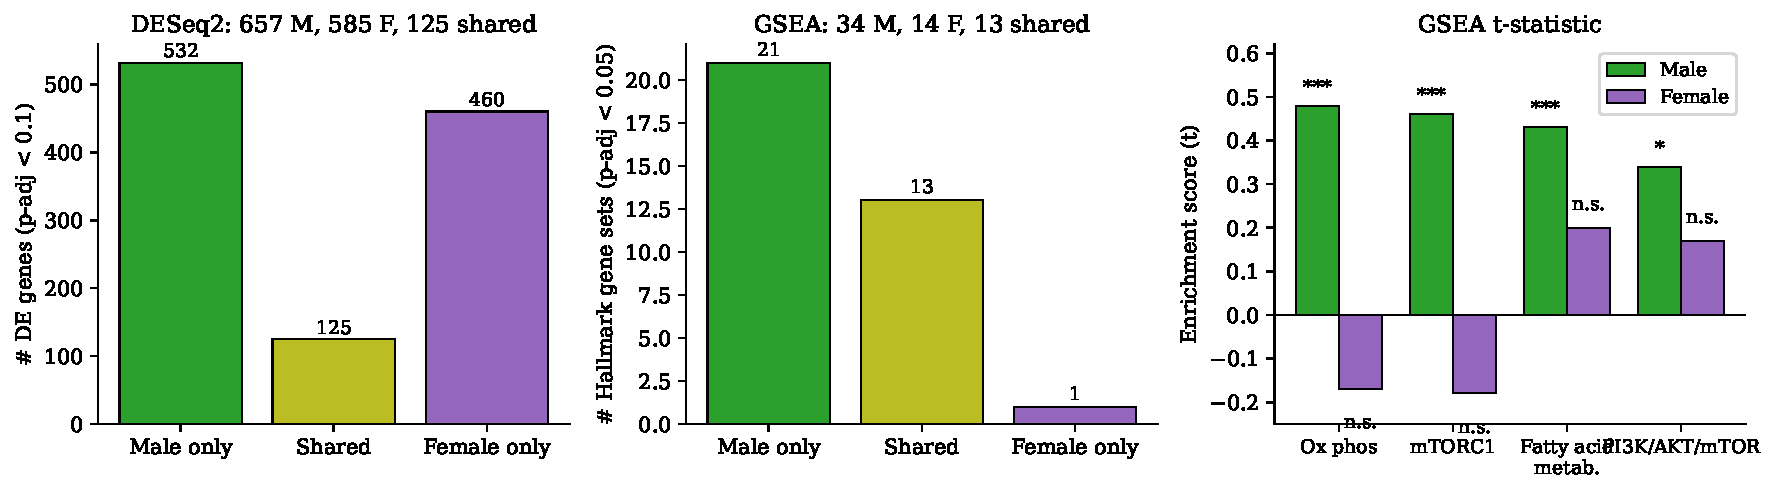
\includegraphics[width=\textwidth]{figures/fig2_rnaseq.pdf}
\caption{Sex-specific transcriptomic response in V1 to food restriction ($n=4$ per group). DESeq2 identified 657 differentially expressed genes in males and 585 in females ($p$-adj~$<0.1$), with 125 shared. Gene Set Enrichment Analysis on Hallmark sets returned 34 significantly regulated sets in males and 14 in females ($p$-adj~$<0.05$), with 13 shared. Canonical energy-regulating pathways showed male-selective enrichment: oxidative phosphorylation ($t=0.48$, $p<0.0001$ in males; $t=-0.17$, $p=0.96$ in females), mTORC1 signalling ($t=0.46$, $p<0.0001$ vs $t=-0.18$, $p=0.98$), fatty acid metabolism ($t=0.43$, $p<0.0001$ vs $t=0.20$, $p=0.88$) and PI3K/AKT/mTOR signalling ($t=0.34$, $p=0.027$ vs $t=0.17$, $p=0.98$).}
\label{fig:rnaseq}
\end{figure}

% Figure 3: ATP usage and orientation selectivity
\begin{figure}[htbp]
\centering
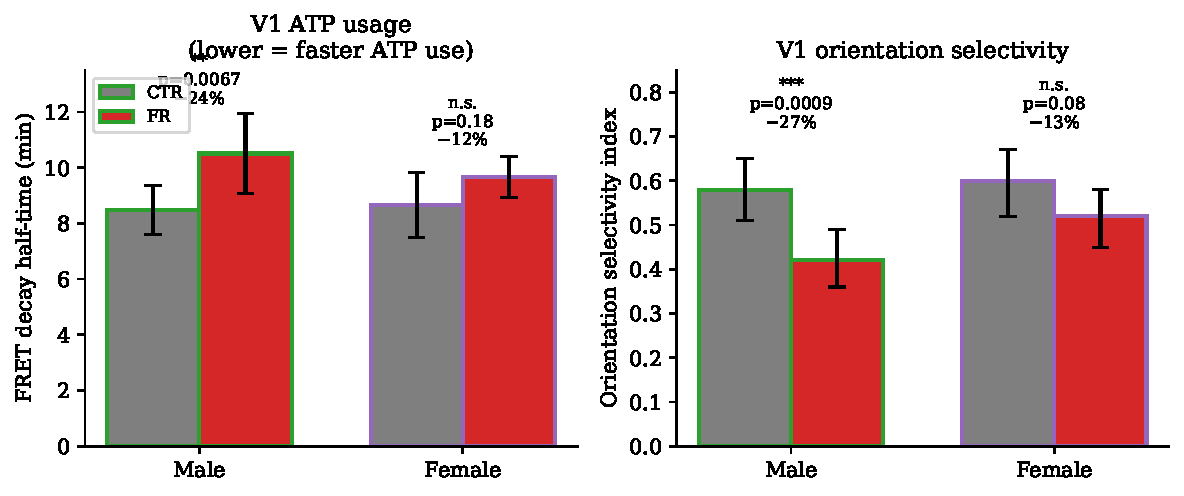
\includegraphics[width=0.9\textwidth]{figures/fig3_atp_osi.pdf}
\caption{V1 ATP usage and orientation selectivity are reduced by food restriction in males but not in females. Left, half-time of FRET decay of the ATeam1.03YEMK signal (shorter half-time = faster ATP usage) during natural-scene visual stimulation. In males, FR slowed ATP use by 24\% (8.48~min [7.59--9.37] to 10.51~min [9.08--11.93]; $t=2.87$, $df=37$, $p=0.0067$; $n=11$ CTR, $10$ FR). In females, the change was 12\% and non-significant (8.66~min [7.49--9.84] to 9.66~min [8.92--10.39]; $t=1.36$, $df=37$, $p=0.18$; $n=12$ CTR, $8$ FR). Right, orientation selectivity index (OSI) from GCaMP6s imaging of V1 layer 2/3 neurons during drifting gratings. Males: 0.58 [0.51--0.65] to 0.42 [0.36--0.49] ($-27\%$; $t=3.75$, $df=27$, $p=0.0009$; $n=8$/$8$). Females: 0.60 [0.52--0.67] to 0.52 [0.45--0.58] ($-13\%$; $t=1.90$, $df=27$, $p=0.08$; $n=7$/$9$). Error bars span 95\% confidence intervals.}
\label{fig:atp_osi}
\end{figure}
